\chapter{Conflict}
\label{app:conflict}
This appendix provides additional information on the conflict data and classification procedures employed in the main analysis \\

We focused on consumption related conflict, filtering the dataset \textcite{acled2025} to include only events not associated with predatory behaviour.\\
This distinction is important because rapacity related events generally reflect violent and opportunistic actions, whereas non rapacity conflicts are more closely linked to income related grievances and economic distress. \\

\begin{figure}[!htbp]
	\centering
	\includegraphics[width=0.8\textwidth]{con.pdf}
	\caption{Dominant conflict type}
	\label{conflitti}
\end{figure}
Figure~\ref{conflitti} illustrates the temporal evolution of conflict events, showing the total number of incidents of each type per year across ADM2 units.\\
Non rapacity conflicts increase sharply after 2015, consistent with the patterns identified in the main analysis, while rapacity events remain relatively stable over time.\\
This divergence suggests that the two categories may be driven, at least in part, by different underlying mechanisms.  \\

\begin{table}[htbp]\centering
	\caption{Panel coverage and sparsity of conflict events}
	\label{tab:panel_coverage}
	\begin{tabular}{lccc}
		\toprule
		\textbf{Conflict type} & \textbf{Average} & \textbf{SD} & \textbf{Peak activity} \\
		\midrule
		Non-rapacity & 0.66 & 2.40 & 336 events in 2020 \\
		Rapacity     & 0.14 & 0.61 & 57 events in 2023 \\
		\bottomrule
	\end{tabular}
\end{table}

Table~\ref{tab:panel_coverage} shows that, on average, each ADM2 experiences almost no conflict events per year.\\
However, the high standard deviation of non-rapacity events reveals substantial heterogeneity across regions, with a few ADM2s concentrating most of the violence.\\
This sparsity and imbalance justify the inclusion of ADM2 fixed effects in the empirical model.

\chapter{Nightlights}
\label{app:nightlights}
This appendix provides additional context on the control variable, nightlights. \\

In the Data chapter we noted visible discontinuities in the series, which \textcite{li2020harmonization} attribute to satellite technology changes and sensor fluctuations. \\
To rule out other drivers, we compared national trends in nightlights with two plausibly related aggregates: conflict intensity (combining rapacity and consumption-related events) and oil–gas rents, given the prominence of minerals and oil in Nigeria’s trade \parencite{imfportwatch2025}.\\

\begin{figure}[!htbp]
	\centering
	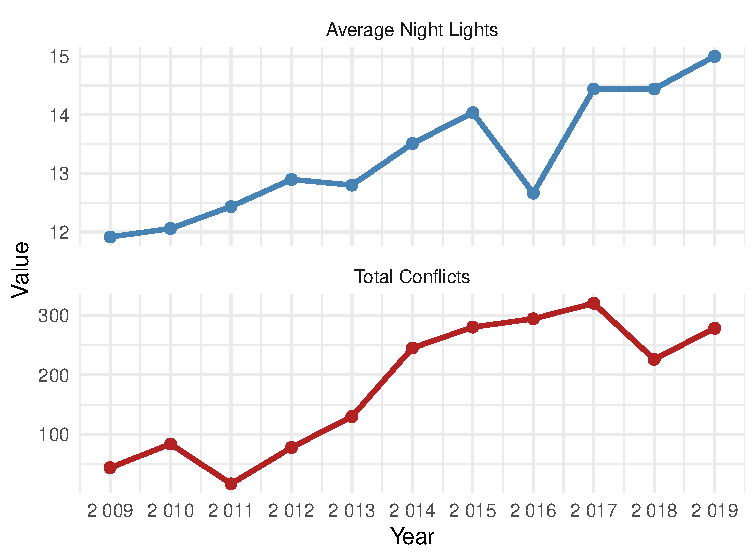
\includegraphics[width=0.8\textwidth]{aa.pdf}
	\caption{Conflict and nightlight}
	\label{nightl}
\end{figure}

\autoref{nightl} shows the patterns are consistent with dual influences. In 2013 and especially 2016, declines in nightlights coincide with marked increases in conflict, suggesting real economic disruption alongside potential measurement noise. \\
\begin{figure}[!htbp]
	\centering
	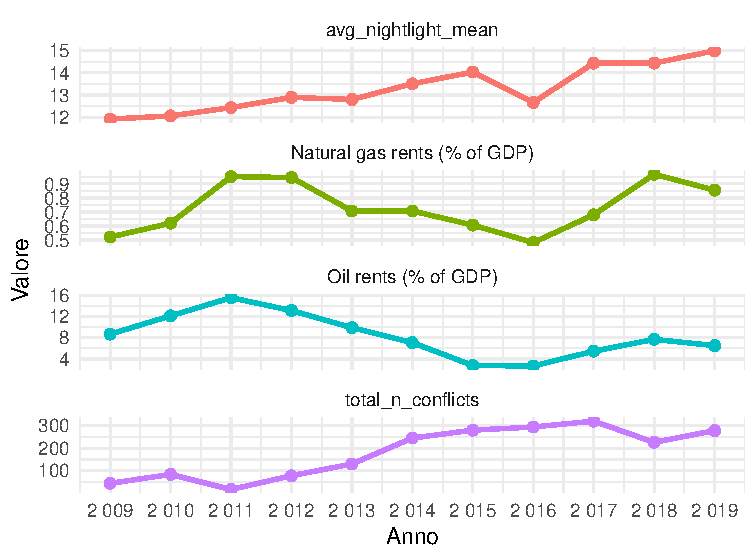
\includegraphics[width=0.8\textwidth]{sec.pdf}
	\caption{Confroning conflict, nightlight and different type of rent}
	\label{con}
\end{figure}

\autoref{con} shows a similar pattern and, in particolar, that the 2016 episode also aligns with a sharp fall in traded-goods rents
Those observations linked with the sensor moviment could explain the drop 
Of course, part of the discontinuity in nightlights reflects known sensor and constellation changes \textcite{li2020harmonization}. Yet the comovement we observe, nightlights falling in 2013 and especially 2016 while conflict rises and traded goods rents contract, suggests a substantive pattern beyond pure measurement noise. This alignment points to plausible real-economy disruption coinciding with the technical break. While we do not claim causality here, the repeated timing and direction of these series indicate a relationship that merits deeper investigation rather than being dismissed as a data artifact alone.
\chapter{Heterogeneity}
\label{app:descriptives}
This appendix provides additional information about the measurement used as heterogeneity employed used in the empirical strategy. \\
In our analyses we accounted for different spatial heterogeneity, in particular for geographic, sectorial, social and environmental one.\\

Starting from geographical dimension, we studied both the differences between East and Ovest and the ones between Nord and South. We costructed the dummies using respectively the longitude and latitude median. Nord and South, as shown in table \ref{tab:ns_summary}, display strong differences in nightlight concentrations, a proxy for economic activity: the South is brighter on average and more dispersed, while the North is dimmer and more stable. This suggests that in southern regions, the wealthiest areas are wealthier than those in the north. \\

\begin{table}[htbp]\centering
	\caption{Summary statistics by North/South macro-region}
	\label{tab:ns_summary}
	\resizebox{1\textwidth}{!}{
	\begin{tabular}{lc|c|c|c|c|c|c}
		\toprule
		Macro-region &$n$ & Mean NTL & SD NTL & Mean trade & SD trade & Mean conflicts & SD conflicts \\
		\midrule
		North & 748  & 1.35 & 0.885 & 9.07    & 50.0     & 0.707 & 1.89 \\
		South & 1232 & 2.59 & 0.932 & 131551.0 & 2782390.0 & 1.19  & 3.55 \\
		\bottomrule
	\end{tabular}
	}
	\vspace{3pt}
	\begin{minipage}{1\textwidth}
	\footnotesize Notes: NTL = log night-time lights. Trade = $indice2\_main$. Conflicts = number of consumption-related events.
	\end{minipage}
\end{table}


However, the corresponding regressions are not statistically significant, so we do not rely on the North/South split in the main analysis. \\
\clearpage
\begin{figure}[!htbp]
	\centering
	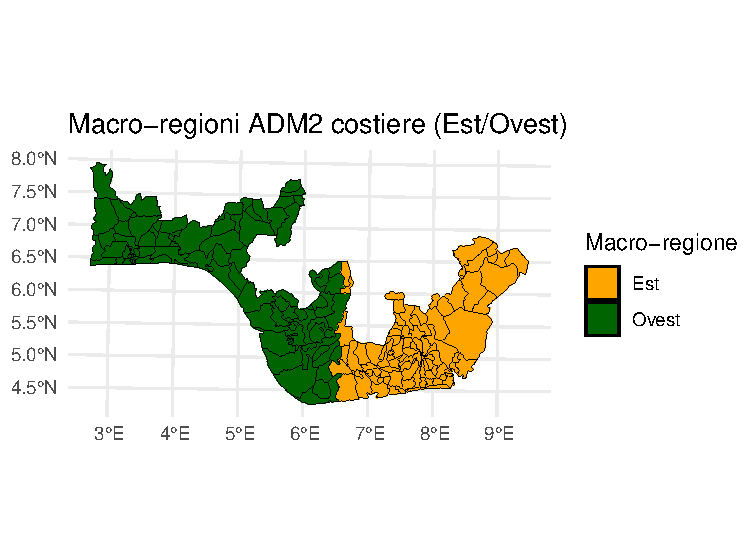
\includegraphics[width=0.7\textwidth]{est_ovest.pdf}
	\caption{est and ovest}
	\label{est}
\end{figure}

We therefore focus on the East West division. Figure \autoref{est} shows the spatial partition and, following the intuition of the Panel B of Table \ref{tab:ns_summary}, we analysed the logarithmic distribution of nightlights by macro region \autoref{est2}.\\

\begin{figure}[!htbp]
	\centering
	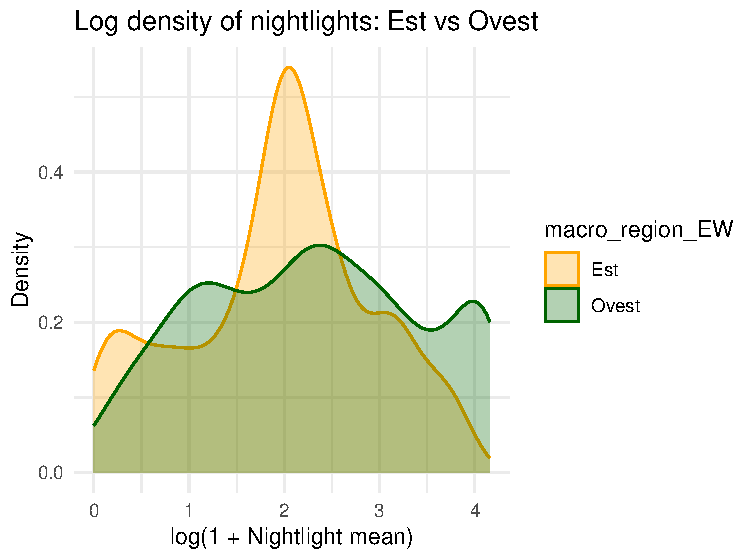
\includegraphics[width=0.7\textwidth]{log est_ovest.pdf}
	\caption{log density of nightlights}
	\label{est2}
\end{figure}
The pattern confirms our intuition: the East, in orange,  concentrates around ~2 with more mass at lower values, while the West, in green, features a heavier right tail up to ~4. This suggest that the western ADM2 units are, on average, brighter and more dispersed.\\

A noteworthy observation is the almost perfect symmetry between the geographic (East/West) and the sectoral dimensions (Import/Export and Vegetables-first/Chemicals-first): they cover largely the same ADM2 units, which strengthens the interpretation of our heterogeneity results.
This symmetries are shown in Figure \ref{est}, \ref{flow} and \ref{sector}


\begin{figure}[!htbp]
	\centering
	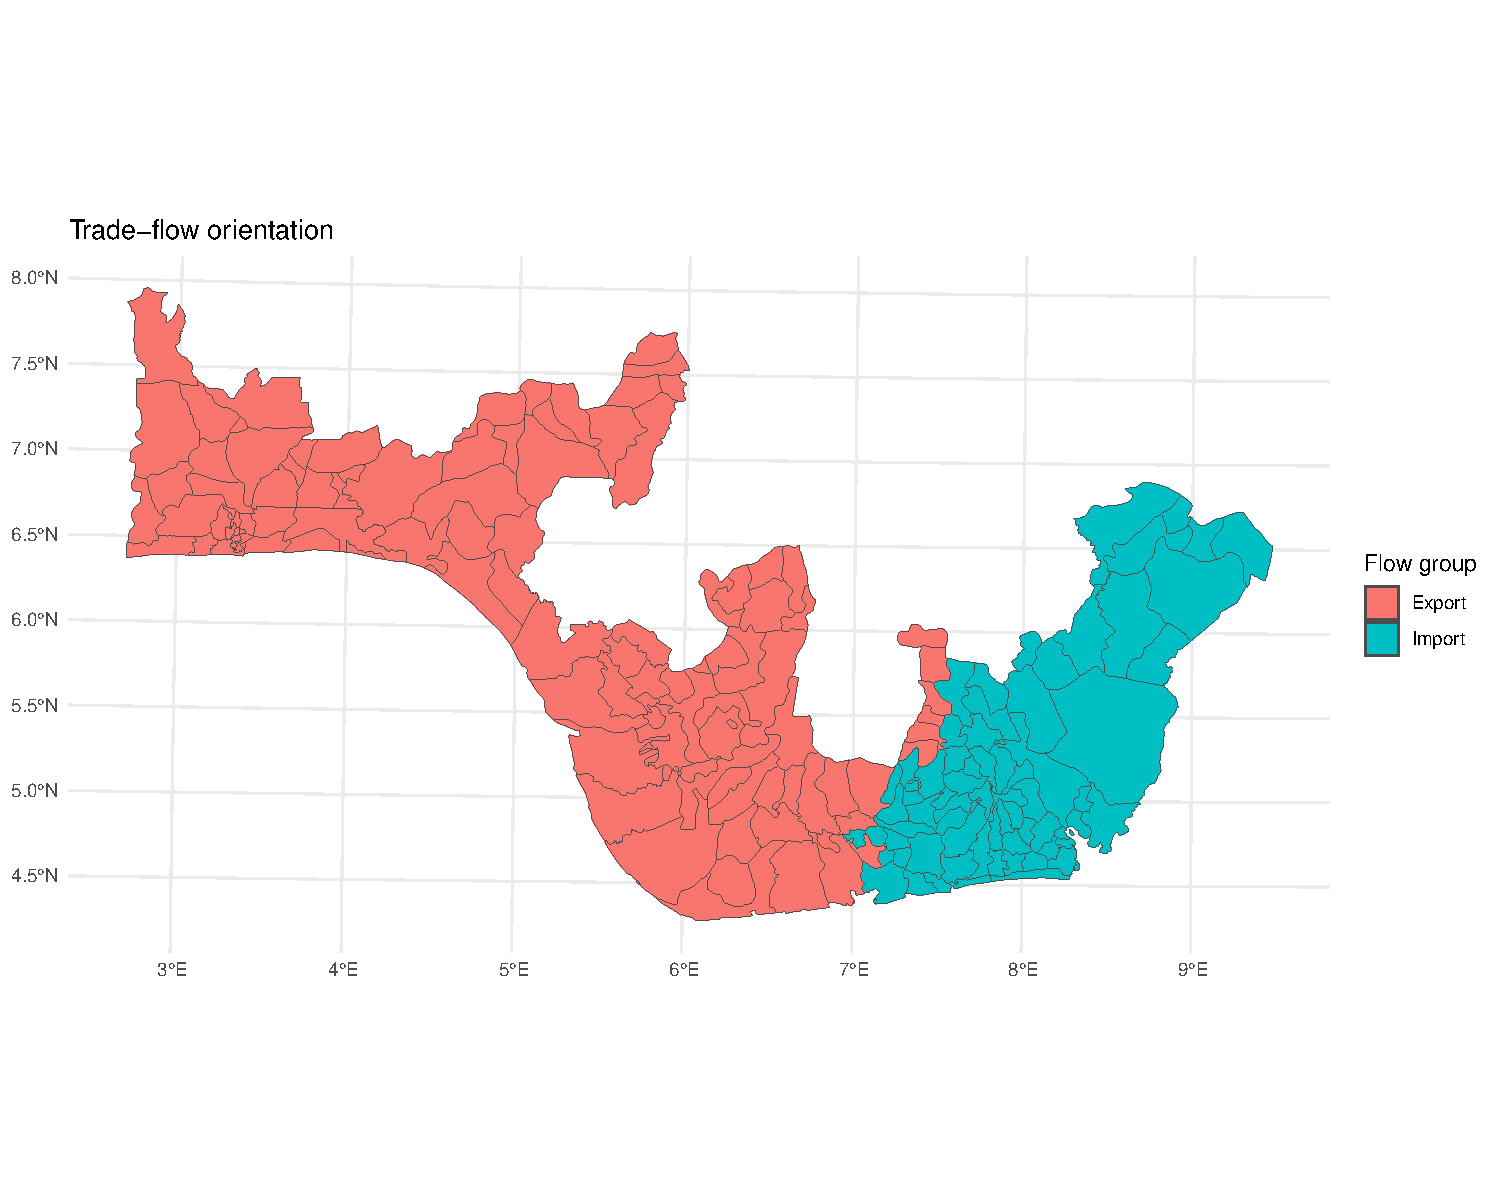
\includegraphics[width=0.7\textwidth]{flow.pdf}
	\caption{Import and export}
	\label{flow}
\end{figure}

\begin{figure}[!htbp]
	\centering
	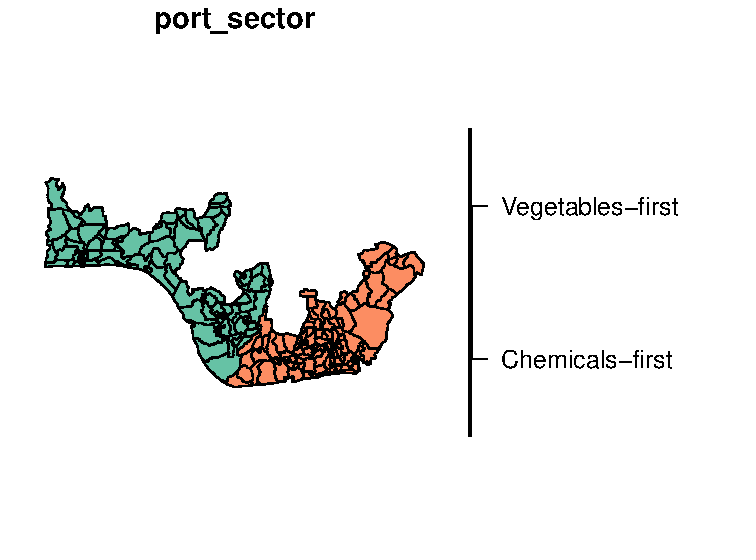
\includegraphics[width=0.7\textwidth]{sector.pdf}
	\caption{Vegetable and chemicals}
	\label{sector}
\end{figure}

\chapter{Replication Code}
% Short intro text (optional)
This appendix provides the R code used to construct the analysis
\lstinputlisting[
language=R,
caption={Full pipeline},
label={lst:pipeline-r}
]{code/main.R}

